\section{General Analysis of Inventory Systems}


We organize and motivate the topics along a set of questions.  The aim
of this approach is to make you think, and discuss with your fellow
students, right away about the fundamental aspects of inventory
theory.  We provide a set of solutions for all the questions to
prevent you from getting stuck.  In case you identify interesting
questions that we do not address, please let us know. Also, when
questions and/or answers are unclear, let us know.

The first relevant question is: why are there actually inventories at
all? Let us analyze this main question by chopping it up into many
small questions and address these questions subsequently. 

We formulate the problems right away in terms of symbols, as this is
much clearer eventually, and will help you implement the models that
we are going to develop in excel, or some more useful programming
environment.


As a guide to the solving the exercises, note that they are not meant
to be easy (otherwise we could have asked you to check that
$11+22=33$\ldots). Thus, it is not a real problem if you can't solve
an exercise right away, in other words, it is not a `failure' if you
are not able to solve an exercise. However, the failure is not to
\emph{attempt} to solve an exercise. Hence, always think hard about an
exercise before you check the solution.  We expect that when you start
on a new exercise you have read, and understood, the solution of all
previous exercises. We urge you to implement all solutions in
excel. Once you know how to do it, it is fairly easy and gives
enormous insight.



Recommended reading:
\begin{itemize}
\item Factory Physics: Section 2.1, 6.3 and  16.2. 
\end{itemize}

\subsection{Inventory Modeling}
\label{sec:inventory-modeling}

\begin{question}\label{ex:1}
  Recall the EOQ formula:
  \begin{equation*}
    Q^* = \sqrt{\frac{ 2 A D}{h}}.
  \end{equation*}
What are the underlying assumptions of the inventory system that lead to this equation?
\begin{solution}
\begin{itemize}
\item Demand is constant and deterministic
\item Lead time is zero
\item Any amount of items necessary to replenish the inventory can be
  ordered
\item There is a cost associated with ordering, no joint-ordering advantages.
\item There is a cost associated with holding inventory
\item Inventory is not perishable.
\item There is no substitution effect with other item types.
\end{itemize}
See also FP.
\end{solution}
\end{question}


\begin{question}
  Can you summarize the assumptions of the EOQ in four steps by which
  a generic inventory system can be characterized?
  \begin{solution}
If we dissect the EOQ model we see that we made modeling decision regarding:
\begin{enumerate}
\item Characteristics of the  demand:  constant, or deterministic, stochastic, trends, seasonality?
\item Models: 
  \begin{itemize}
  \item Characteristics of the replenishment structure and properties
    of the items.
  \begin{itemize}
  \item  are items produced or ordered, do we deal with a FGI or a RMI? 
  \item is the order size unlimited or bounded (for instance by
    production capacity)? 
  \item Is the lead time positive or not?
  \item Are the items perishable or not?
  \item the number of items, e.g., are we concerned with ordering just
  one item type or more? In case of the latter, can orders be joined
  or not? How many suppliers do we have?
  \end{itemize}
\item the cost structure, e.g., 
  \begin{itemize}
  \item is there cost associated to lost  demand, backlogged demand, inventory?
  \item costs associated to the ordering and/or production (set up
    cost, setup time)
  \item KPI's.
  \end{itemize}
\end{itemize}
\item Policies to control of the inventory. What type of policy to use? 
\item A specification of the policy parameters and a sensitivity
  analysis of the EOQ formula (see FP).
\end{enumerate}
  \end{solution}
\end{question}

\begin{question}
  Why is it important to make a model of an inventory system?
  \begin{solution}
    \begin{itemize}
    \item With a model it becomes possible to actually manage an
      inventory system. The model included the basic, and most
      revelation, relations between the different parts of the system.
    \item A model can help with consistency checks. For instance,
      suppose we order in quantities of $Q$, e.g., 100 items, what is
      the implied ordering cost?  Well: use the EOQ formula to see
      that this is $A=hQ^2/2D$.  Lets suppose that $h=1$ Euro per year
      per item, and the demand is 100 items per year. Then,
      $A=1(100)^2/(2\cdot 100) = 50$ Euro. Depending on the business
      context this may reasonable, in the order of a delivery cost by
      a truck.
    \item With models we can carry out simulations with the aim to
      evaluate the consequences of using certain types of control
      policies, when to order, and how much to order.
    \item With models we can carry out sensitivity analysis. How
      sensitive is our policy with respect to changed in the cost
      parameters, demand, and so on? Suppose it turns out that the
      costs are very sensitive, it is important to monitor the
      inventory levels/positions closely, for instance, continuous
      review may be necessary. if it is not so sensitive, periodic
      review can be OK.
    \item Finally, we can use models for what if scenarios.  We can
      investigate what happens if we change (some of) the assumptions
      underlying the model and develop methods to assess inventory
      control policies. With a model we can also analyze hypothetical
      situations and the efficacy of certain types of policies to
      avoid undesirable situations. (In fact, we use such models to
      try to understand how we can avoid ending up in a certain
      situation we never want to enter in reality.)
    \end{itemize}
  \end{solution}
\end{question}

Hopefully the above questions and answers provide sufficient
motivation for the next few lectures in which we develop
\begin{enumerate}
 \item models of inventory systems  and policies. 
 \item models to characterize demand and make forecasts of demand
\end{enumerate}
Mind that you also have to carry out these steps in the group
assignment.


\subsection{Analyzing Inventory Systems}
\label{sec:analyz-invent-syst}

Before making models of inventory systems we need to get an
understanding of the most relevant parts of inventory systems.  For
this purpose, lets start from the basics and see how far we get by
asking (relevant) questions.  The most basic question is actually:
`Why do we need inventory at all?', so that question will be our point
of departure.

\begin{question}
  When are inventory systems actually not necessary?
\begin{solution}
  In a sense, in business it comes down to matching supply and
  demand. When capacity can be modulated at will and free of cost,
  there is not need for inventory. Any demand size be produced or
  ordered without any problem and without any financial consequence.

  The problem is of course that these two conditions are (nearly)
  never met in real systems.
\end{solution}
\end{question}



\begin{question}
When, then, are inventories necessary?
  \begin{solution}
    In real systems there are many constraints imposed on replenishing
    the inventory which makes matching supply and demand
    complicated.

    In case of FGI, production limitations (production typically has
    finite production speed, and works in batches because of setups),
    demand cannot be served when it arrives.  In case of RMI, we need
    to respect supplier and transportation characteristics, so that we
    cannot order any quantity we like, and we need to take into
    account replenishment lead times. There can also be other
    constraints, for instance the supply can be only seasonable, e.g.,
    wheat.

    The items sold to customers has constraints such as the amounts in
    which it is produced, it can be perishable or not.

    The demand has constraints: customers may not be prepared to wait
    (backlogged), or it actually physically impossible to backlog
    demand. Demand can be lost if not met right away. Thus, a certain
    service level might need to be met.

    
    There are costs associated with all these constraints: ordering
    cost, holding cost, production costs, backlogging cost, lost
    sales, and so on.

    In this setting, with all these constraints, it is necessary to
    make trade-offs. Cost minimization then, typically, leads to
    installing inventories, since with inventories costs can be lower
    as compared to a system without an inventory. 


    In fact, even if it technically possible to match supply and
    demand perfectly, there may be very high costs associated with the
    achieving this perfect match. Thus, in such cases, inventories are
    also used  to lower costs.
  \end{solution}
\end{question}


\begin{question}
Thus, all-in-all, what is the goal of the inventory system?
  \begin{solution}
    Inventory systems exist out of economic necessity. They are meant
    to reduce the cost of operations. 
  \end{solution}
\end{question}


\begin{question}
  So, taking the idea of the previous exercise seriously, i.e.,
  inventory systems are meant to lower the cost of operations of the
  firm, we like to know how to do this. This brings us to the idea of
  making a model of an inventory system to characterize the demand,
  replenishments, items and the cost structure. Try to formulate a
  sort of checklist which can help to carry out this modeling step.
  \begin{solution}
    In effect, the problem is to come up with a guide to making
    inventory models.  A useful starting point is formed by the four
    stages of our inventory analysis scheme.  For each stage we
    formulate a set of (yes/no) questions. Of course this list will not
    be complete (it can never be complete, life is too varied for
    this\ldots), but it can capture at least a number of important aspects.
    \begin{enumerate}
    \item Demand characterization:
      \begin{itemize}
      \item Can customers wait or not?  If so, how long? Is there a
        cost, like registration, associated with putting demand into
        backlog? Is there a cost associated with duration of waiting?
      \item Can demand be lost? If so, to what extent, e.g., 5\%? What
        is the cost of loss, or forgone revenue?
      \item Is demand more or less constant, or (very) stochastic? Trends, seasonality?
      \end{itemize}
    \item Supply, replenishment characteristics
      \begin{itemize}
      \item FGI:
      \begin{itemize}
      \item can production be switched on and off?  Is there a cost
        associated with switching capacity on and off
      \item What is the production speed?
      \item Does production work in complete batches, or can it produce single items?
      \item Do we have to deal with MTO or MTS production? 
      \item Where to locate the I/O interface?
      \end{itemize}
    \item RMI:
      \begin{itemize}
      \item Is there a size constraint on the amount that can be ordered? 
      \item Is there a lead time between ordering and receiving the
        replenishment? Is the lead constant, variable, stochastic?
        Does it change over time?
      \item Is yield loss (i.e., we can not use all of the items that
        the supplier delivered) relevant ?
      \item Are orders always on time?
      \item Are items ordered jointly with other items, joint
        replenishments?
      \item Is there a cost associated with ordering? Is there a fixed
        and/or and variable part of this cost? Quantity discounts?
      \item Single or multiple suppliers?
      \end{itemize}
    \item Items:
      \begin{itemize}
      \item Are items held at one single-echelon, or in a
        multi-echelon system?
      \item holding costs?
      \item Deterioration,  perishability cost? 
      \item single-item or  multi-item
      \item budget and/or warehouse limitations
 \end{itemize}
      \end{itemize}
    \item Policy selection:
      \begin{itemize}
      \item What do we want to achieve? Satisfy a service level
        constraint, or minimize cost? In case of the latter, do we
        want to minimize cost over one or many periods?
      \item Periodic or continuous review?
      \item What decisions/controls are at our disposal to affect the
        behavior of the system, hence affect the cost?
      \item What properties do we require? Should it be simple?
        Operate it manually, or by computer? 
      \end{itemize}
    \item Policy evaluation:
      \begin{itemize}
      \item What KPIs are important? What customer service level do we
        need, e.g., fill rate, cycle-service level.
      \item How to position/relate all cost components with respect to
        each other?
      \end{itemize}
    \end{enumerate}
  \end{solution}



See Figure~\ref{fig:costs} for a visual overview.

\begin{figure}
\centering
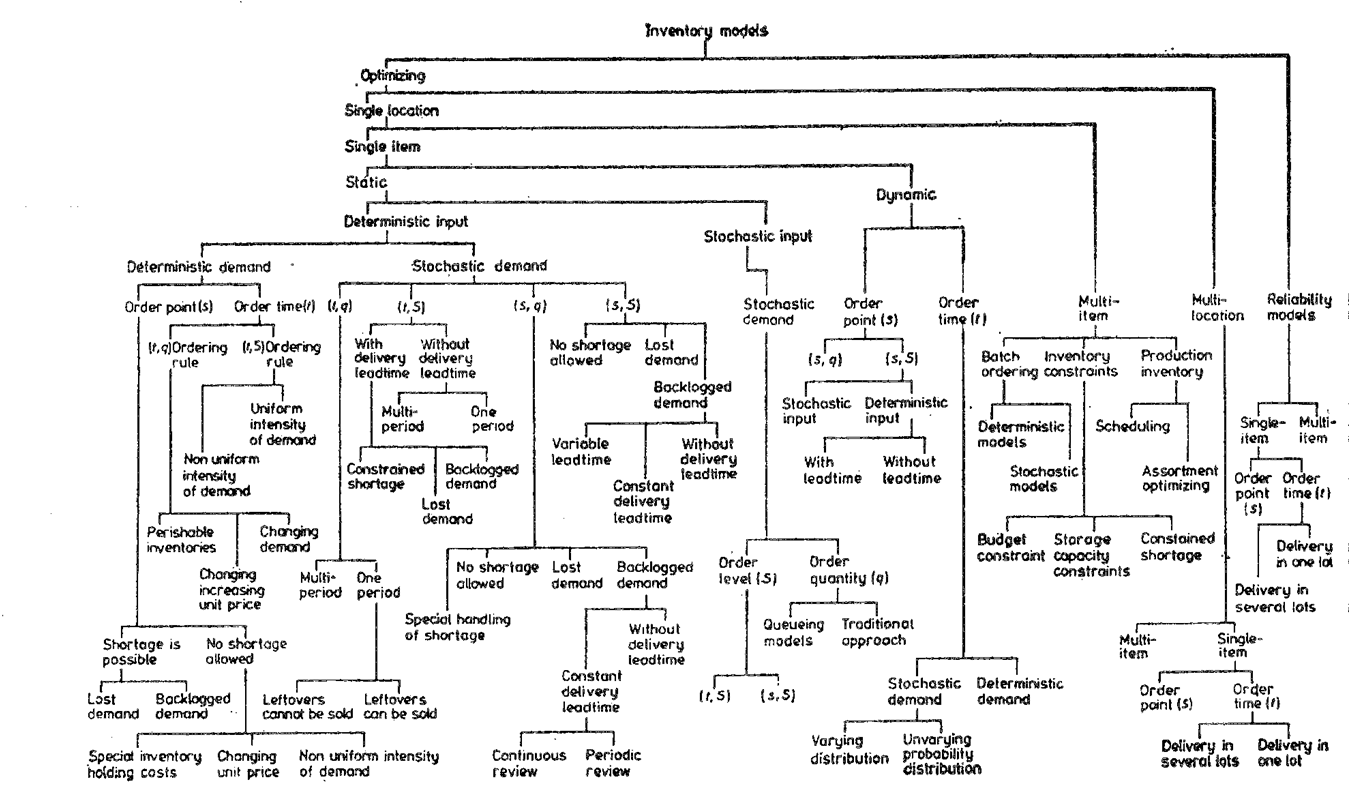
\includegraphics[width=\textwidth]{figures/chikan.png}
\caption{Decomposition of inventory models}
\label{fig:costs}
\end{figure}


\end{question}



\begin{question}
  Clearly, to make decisions it is important to have a good understanding
  of the relevant trade-offs. Interestingly, all these trade-offs can
  be reduced to three types of buffer. What buffers can that be?
  \begin{solution}
    Time, inventory, capacity, the three buffers. We urge you to read
    Section 6.2 and 6.3 of FP (edition 3) really critically. The ideas
    behind Figure 6.6 are very useful, and you can try to apply the
    underlying ideas to your case too when you have to make a choice
    for an inventory control policy, determine the policy parameter
    and do the sensitivity analysis.
  \end{solution}
\end{question}



\subsection{Modeling Examples}
\label{sec:examples}

We'll now use the check list we developed in one of the exercises
above to analyze a few simple inventory systems. We'll make a model
first, with symbols, because this helps in the communication about the
model and the documentation. Once we have a complete model we can
build it in excel and start simulating the system and evaluate
policies. Thus, the aim of the examples is to show you how to apply
the check lists to design and evaluate complete models. Note that
modeling is an art; as a consequence check lists can never be
complete, and there is also not one simple recipe to make a good
model. In that sense, the development of models is always somewhat
ad-hoc and unstructured, in fact, the development of the model helps
you to familiarize yourself with a situation you don't completely
understand. There is no way around except that you start modeling,
accept to make mistakes in the process, and test your assumptions and
modeling decision, improve your model after these test, and so on. The
proof of the pudding is in the eating\ldots and you don't know upfront
whether your model will be correct or not.

So we start with making a very simple model, a case description if you
will, and make it more complicated as we go along.  You are supposed
to follow the steps and implement them in excel, make graphs, compute
KPIs, and so on, to test your understanding of the approach to problem
solving we want you to learn.

\subsubsection{Systems with Backlog but without Inventory on hand}

\begin{question}
  Consider a production situation, a  machine for instance, that has a
  production capacity of  $c$ per day, e.g. $c=10$.  The daily demand,
  $d_i$ for day $i$, is always less then $c$. Is there a need for inventory?
  \begin{solution}
No, since $c\geq d_i$, the daily demand can be covered by production every day again.     
  \end{solution}
\end{question}

\begin{question}
  Let's assume that the machine can be switched on or off.  If on, it
  has capacity for $c$ jobs, if off it produces nothing.  Just to show
  the impact of the cost structure on the policy you would use to
  control the machine, suppose that the cost to operate the machine is
  $p$ per job, i.e., you only have to pay for the jobs you really
  processed. What what you do, that is, how would you control the
  machine?
  \begin{solution}
    Well, since it only costs money per job served, and we want to
    serve the jobs anyway, we can just switch on the machine whenever
    there is a job. In fact, we can leave it on always, for there is
    no penalty to have it switched on (or a reward for switching it
    off).
  \end{solution}
\end{question}

\begin{question}
  Henceforth we assume that it costs $p$ Euro per day, for instance
  $p=100$ euro, just to have the machine switched on, whether you use
  the capacity or not. What would you do now? When is such cost structure reasonable?
  \begin{solution}
    If $d_i=c$, i.e., the daily demand is always the same as the daily
    capacity, then there is not much you can do. However, if the
    demand is typically less than $c$, then it might be interesting to
    occasionally switch on the machine and let it produce all demand
    up to some time. That is, ensure that the machine capacity $c$ can
    be completely used when it is switched on. 

    If you have to hire or assign personel to operate the machine, you
    are typically confronted with a daily cost, whether the machine
    actually works or not.
  \end{solution}
\end{question}



\begin{question}
  Try to make a model for this case.  Use the check list to see what
  modeling choices you can (and have to) make.
  \begin{solution}
    Assume that customers are willing to wait for free.  Assume also
    that we want to serve all demand. (Note that this is a business
    decision. It might be profitable to reject some demand. ) Finally,
    assume that the demand process $\{d_i, i=1,2\ldots\}$ is given.

    You should realize at this point that capacity has a
    `lose-it-or-use-it' property. Unused capacity is lost, and any
    cost associated with that lost capacity is also lost.

    The best thing we can do then is to only switch on the machine
    when the total accumulated demand is larger than the capacity for
    a day.  Thus, if $d_1=2, d_2 = 5, d_3 = 4$, then take the capacity
    $c_1$ for day 1 equal to 0, and likewise for day 2. However,
    $c_3 =10$. 
  \end{solution}
\end{question}


\begin{question}
  Implement the model in excel, and compute the total cost for the
  following demand process: $d = 2, 5, 4, 5, 0, 2, 3, 8, 9, 1, 1, 3$.
\begin{solution}
  Take $c_i$ as the capacity of day $i$. In our case $c_i=c=10$ if
  production is on, and $c_i=0$ if production is off.  Realize that
  any unfilled demand is transferred to the next period. To keep track
  of total demand, let's call $B_i$ the total demand in the system
  waiting for the machine to make their item. Then, if the machine
  does not produce anything in day $i$, the unfulfilled demand at the
  end of day $i$ is $B_i=B_{i-1}+d_i$, i.e., we start day $i$ with
  unfulfilled demand $B_{i-1}$ and then the demand $d_i$ arrives on
  day $i$. On the other hand, if the machine does produce, the total
  unfulfilled demand is $B_i = B_{i-1}-10 + d_i$, since we produce
  10. Thus, in general,
  \begin{equation*}
    B_i = B_{i-1} + d_i - c_i.
  \end{equation*}


  Typically, the unfulfilled demand is called \emph{backlog}. The
  interpretation is really simple, it is exactly the same as the queue
  of customers waiting for capacity. If you would apply this reasoning
  to the number of customers in queue waiting in a supermarket for
  service you would obtain exactly the same result.  

Thus, once and for all, backlogged customers, or backorders, are precisely the same thing as a queue of jobs or customers waiting for capacity. 

Realize also that this equation can be implemented straightaway in
excel.

Finally, observe that in the above we assume that when the machine is
on at day $i$, the capacity $c_i \leq B_{i-1}+d_i$, because otherwise
the $B_i<0$, and it is impossible to have a negative number of
customers in queue/backlog.
\end{solution}
\end{question}


\begin{question}
  Now we have to make a subtle choice. It might not be possible to use
  the capacity on day $i$ to handle the demand $d_i$ that arrives on
  day $i$. Of course, it also might be possible. In general it depends
  on the actual characteristics of the system which of the two
  assumptions is the more appropriate.  How would you absorb these
  choices into your model?
  \begin{solution}
    Suppose that the demand that arrives at day $i$ can also be covered by the machine in day $i$. It that case we only need to require that 
    \begin{equation*}
    B_i = \max\{B_{i-1} + d_i - c_i, 0\}.
    \end{equation*}
    Like this we are sure that the number of jobs in backlog is not
    negative.  

Otherwise, if the demand on day $i$ has to wait at least until day $i+1$, then
    \begin{equation*}
    B_i = \max\{B_{i-1} - c_i, 0\} + d_i.
    \end{equation*}

    Fill in these formulas with a set of numbers for the demand and
    implement it in excel to see what happens.  Start doing all kinds
    of experiments. How sensitive is the result to changes in $c$, for
    instance? What is a good rule to switch on and off the machine?
  \end{solution}
\end{question}

 


\begin{question}
  Can you find a set of formulas by which we can track the behavior of the backlog? 
  \begin{solution}
    Lets say that $S_i$ is the amount of demand sold/covered on day $i$. Henceforth we also assume that the demand on day $i$ \emph{can} be processed on day $i$. In this case, the amount sold is 
    \begin{equation*}
      S_i = \min\{B_{i-1}+d_i, c_i\},
    \end{equation*}
    since we cannot produce/sell more than the demand in backlog and
    we can also not sell more than the capacity.  The backlog is therefore,
\begin{equation*}
  B_i = B_{i-1}+d_i - S_i.
\end{equation*}
  \end{solution}
\end{question}

\begin{question}
  Suppose that we would decide to switch on the machine independently
  of the amount of jobs. Can you find a formula, to be implemented in
  excel, to compute the amount of capacity lost?
  \begin{solution}
The unused capacity $U_i$ is then
\begin{equation*}
  U_i = c_i - S_i,
\end{equation*}
because $c_i$ is the capacity we have, and $S_i$ is the amount we
used.

It is very important to memorize this scheme. Hence, once again:
\begin{align*}
      S_i &= \min\{B_{i-1}+d_i, c_i\}, \\
  U_i &= c_i - S_i, \\
  B_i &= B_{i-1}+d_i - S_i.
\end{align*}
Note that this scheme is quite simple in the sense that we have to
consider taking a minimum only once. 

  \end{solution}
\end{question}



\begin{question}
  For the rest of the course we need some important notation. What is the meaning of $\sum_{i=1}^j x_i$, and why is $h \sum_{i=1}^j x_i = \sum_{i=1}^j (hx_i)?$
  \begin{solution}
    \begin{align*}
      \sum_{i=1}^3 x_i &= x_1 + x_2 + x_3 \\
      \sum_{i=1}^j x_i &= x_1 + x_2 + \cdots +x_j \\
     h \sum_{i=1}^j x_i &= h(x_1 + x_2 + \cdots +x_j) = hx_1 + \cdots+hx_j = \sum_{i=1}^j h x_i.
    \end{align*}
  \end{solution}
\end{question}

\begin{question}
  Realize that in the previous problem we tacitly assumed that there
  is no cost associated with waiting.  In this case, we of course only
  switch on the machine when there is sufficient demand in
  backlog. But what would you do if there is a cost of waiting, for
  instance, if it costs $b$ per day to keep one unit of demand
  waiting. Then it might not be so efficient, in terms of costs, to
  only switch on the machine when the demand is sufficiently high to
  prevent lost capacity. Can you find an expression for the cost of
  keeping demand waiting and switching on the machine?
  \begin{solution}
    In excel we can build something really useful, the indicator
    function. It is 1 if $c_i>0$ and $0$ when $c_i=0$. Mathematically
    we write it like $1\{c_i>0\}$.  

    With this it is easy to compute the total cost up to some day
    $j$. On day $i$ we pay $b B_i$ if there are $B_j$ units of demand
    in backlog, and we pay $p 1\{c_i>0\}$ for the production. Thus,  the total cost up to time $j$ must be 
    \begin{equation*}
      b\sum_{i=1}^j B_j + p \sum_{i=1}^j 1\{c_i > 0\}.
    \end{equation*}

  \end{solution}
\end{question}

\begin{question}
  Assume next that we get a profit $r$ per unit demand sold/produced, then
formulate the reward structure.
  \begin{solution}
    The profit function up to time $j$ is
    \begin{equation*}
     r \sum_{i=1}^j S_j - b \sum_{i=1}^j B_j - p \sum_{i=1}^j 1\{c_i>0\}, 
    \end{equation*}
    i.e., the sum of the total profit minus the cost of backlog minus
    the cost of switching on the machine (recall $c_i = 0$ is the
    machine is off and $c_i = 10$ if on.).

  \end{solution}
\end{question}

\begin{question}
  It might be that the business context requires that the amount of
  backlogged demand should not exceed some critical level $a$ say too
  often. Can you find an expression to estimate how often such an
  event occurs with excel for a given set of demands?
  \begin{solution}
    When $B_i>a$ we are `in trouble. Thus, to count how often this happen, we can compute
    \begin{equation*}
      \sum_{i=1}^j 1 \{B_i > a\}.
    \end{equation*}
  \end{solution}
\end{question}

\begin{question}
  Observe that in the previous exercise we only counted the number of
  periods in which the backlogged demand exceeded some level $a$. It
  might also be of interested to compute the total amount of
excess  backlogged demand. What can be an appropriate formula for this? 
\begin{solution}
    When $B_i>a$, the amount in excess is $B_i$. Thus, 
    \begin{equation*}
      \sum_{i=1}^j B_i 1 \{B_i > a\},
    \end{equation*}
  is the amount we want to compute. 
\end{solution}
\end{question}

\begin{question}
  What is the total amount of demand backlogged? 
  \begin{solution}
    In the previous expression set $a=0$. 
  \end{solution}
\end{question}

\begin{question}
  If you like, you can try to formulate an optimization problem for
  the problem on how much to produce. .
  \begin{solution}

    TBD = to be done = unfinished. You can always skip exercises that
    are marked as TBD.

The decision variables are whether we switch on the machine at the days, i.e., $c_1, c_2, \ldots, c_j$. 

The constraints are:

\begin{align*}
c_i &\in \{0, 10\}, \\
      S_i &= \min\{B_{i-1}+d_i, c_i\}, \\
  B_i &= B_{i-1}+d_i - S_i.
\end{align*}

In Section 16.2 of Factory Physics it is shown how to optimize this
problem in excel for \emph{given} demand, i.e., if we know the
demands.  If we don't know the demands, then things become quite a bit
different.

  \end{solution}
\end{question}



\subsection{Systems with Inventories}
\label{sec:inventories}

\begin{question}
  In the previous problem we tacitly assumed that customers are
  prepared to wait.  What if this is not the case, i.e., you serve
  them right away, or they leave. Suppose we don't want demand to
  leave. What can you do about this?
  \begin{solution}
    We assumed that demand arriving on a day cannot be covered/served
    on that same day. If we don't have inventories, all demand will be
    lost. Thus, the only way out seems to be to start keeping real
    inventories. (Realize that up to now we only considered backlogged
    demand, which is, in a sense, negative inventory.) 
  \end{solution}
\end{question}

\begin{question}
  So, let us assume for the remainder that it is possible to invest in
  inventory. How much inventory do we need? Assume that the production
  of the machine can be used to satisfy the demand for that day. 
  \begin{solution}
    If we don't want to lose any demand, and if demand is capped by
    some number, e.g.  $\bar d$ is such that $d_i \leq \bar d$ for all
    $i$, then we are always safe by keeping $\bar d$ items on hand,
    i.e., $\bar d-c$ on shelf at the start of the day
  \end{solution}
\end{question}

\begin{question}
  Write $I_i$ for the inventory at the end of day $i$.  
% We now need to
%   make an assumption about how $\bar d$ compares to the maximal
%   machine capacity $c$. 
  Let us also we assume that $\bar d \leq c$ (that is, the machine can
  always produce more than the maximal demand).  Use this to come up
  with a rule to decide when to switch on the machine.
  \begin{solution}
    We need at the start of the day an inventory of $\bar d$ to cover
    the demand. Realize that the inventory at the start of the day is
    the same as the inventory at the end of the previous
    day. Therefore, for day $i$ we want that $I_{i-1} = \bar d$. If,
    however, $I_{i-1}<\bar d$, we need to produce. But now recall that
    what we produce on a day cannot be used to serve the demand for
    that day.  Thus, we need to prevent that $I_{i-1}<\bar d$, because
    if that happens, we might be one day too late.

    Realize that also that, by assumption, the machine has sufficient
    capacity to cover the maximal demand of one day. Thus, we are safe
    if we produce whenever $I_{i-1} <2 \bar d$, and we don't have to
    be concerned with loss.  

All in all, 
    \begin{align*}
      c_i &= c1\{I_{i-1}< 2\bar d\}, \\
      I_i &= I_{i-1} -d_i + c_i. 
    \end{align*}
  \end{solution}
\end{question}

\begin{question}
  Try to make a cost model. Assume that we charge for inventory at the
  end of the day.  There is a cost $h$ to have one item on hand at the
  end of the day.
  \begin{solution}
    The cost of inventory is $\sum_{i=1}^j h I_{i}$ and the cost of
    production has been given before: $p\sum_{i=1}^j 1\{c_i>0\}$.

    Observer there is no backlog, and also no lost demand. Hence,
    these terms do not add to the cost.
  \end{solution}
\end{question}

\begin{question}
  If, however, $c< \bar d$, the situation changes quite
  dramatically. Suddenly, to prevent loss we need more than $\bar d$
  of inventory at the start of the day, because if the inventory
  becomes below $\bar d$, we might not be able to replenish it
  sufficiently for the next day. What would you do?
  \begin{solution}
    First of all, we observe that it is impossible to prevent lost
    sales under all circumstances if demand is stochastic. It can
    happen that we have 10 days in row, say, that the maximal demand
    arrives. We need already quite a bit of inventory to cope with
    this. In general, in case demand is stochastic, any amount of
    demand can arrive, so that we cannot protect ourselves always
    against loss. 

    Thus, we need \emph{safety stock} to compensate for the fact that
    our production cannot cope with the maximal daily demand.

    We also need to assume that the capacity of the machine is higher
    than the average demand, for otherwise we will have quite a bit of
    loss. 

    Tuning the safety stock to minimize cost is an issue we'll address
    next. 


  \end{solution}
\end{question}

\begin{question}
  What would happen if there is a number of periods between the moment
  the items are produced and that the items become available for
  sale.  How would you organize your production plan, i.e., the periods in which to to decice to switch on the machine? 
  \begin{solution}
    TBD.
  \end{solution}
\end{question}

\begin{question}
  Can you relate the production of the machine to a situation in which
  inventory is replenished by a supplier?
  \begin{solution}
    The production amount $c$ is equivalent to a constraint on the
    amount that can be ordered from a supplier. The time between
    deciding to produce and the moment an item is available for
    customers is equivalent to a lead-time between ordering a
    replenishment order and receiving the replenishment.
  \end{solution}
\end{question}

\subsection{Systems with loss}
\label{sec:real-that-prev}

\begin{question}
  Lets step back a bit\ldots In fact, we do not need to keep at least
  $\bar d$ items of on hand inventory. What if we would carry less
  inventory, and accept a bit of loss?  After all, the cost may
  decrease if we allow for this situation. Can you make a model for
  this situation, that is, a model that can cope with loss?
  \begin{solution}
    This is an interesting situation. First assume there is no
    loss. Then the total amount we produce is the same as the total
    demand. The production cost, i.e., cost to switch on the machine
    is relatively simple. It is just the total demand divided by the
    daily production capacity $c$ and then times the production cost
    $p$ per day, in other words, the total cost of production is
    $p\sum_{i=1}^j d_i/c$.

    If there is loss, however, we need to produce less (because some
    demand is lost) and we also can keep lower inventories. Thus,
    accepting a bit of loss may be interesting as we get cost
    reductions in two aspects: less production and lower inventories.

    A simple policy is to switch on production when the inventory
    $I_{i-1}\leq r$ for some (base-stock) level $r$. 

Observe also that our sales $S_i$ in day $i$ may need not be equal to the demand $d_i$,  as we cannot sell more than what we have on stock. Thus,
    \begin{align*}
      c_i &= c 1\{I_{i-1} \leq r\}, \\
      S_i &= \min\{d_i, I_{i-1}\}, \\
      L_i &= d_i - S_i, \\
      I_i &= I_{i-1} -S_i + c_i, 
    \end{align*}
    where $L_i$ is the lost demand. Note that as $S_i \leq d_i$,
    $L_i \geq 0$ (i.e., we don't run into the trouble of negative lost
    demand).
  \end{solution}
\end{question}

\begin{question}
  What would be the cost of this situation, assuming that it costs $k$
  per unit of demand lost? 
\begin{solution}
  \begin{equation*}
    \sum_{i=1}^j \left(h I_{i} + k L_i + p1\{c_i>0\}\right).
  \end{equation*}
\end{solution}
\end{question}

\begin{question}
  How would you use the results of the previous two exercises to tackle the case in which the machine capacity is less than $\bar d$?
  \begin{solution}
    As a matter of fact, we don't have to change anything. We can use
    the results right away. Observe that the control parameter is $r$,
    i.e., the re-order level. By trying different choices for $r$ we
    can compute/simulate the inventory level, loss and so on, and the
    total cost. The best $r$ minimizes this cost.

    Realize that, formaly, it is not necessary that $c$ is larger than
    the mean demand. If it is less, simply more loss will occur.
  \end{solution}
\end{question}


\begin{question}
  Use the numbers $\{L_i\}$ and $\{S_i\}$ to estimate the fill rate,
  the loss rate, and the service cycle level.
\begin{solution}
The total demand is
\begin{equation*}
 \sum_{i=1}^j d_i, 
\end{equation*}
and the total amount of demand served/sold is 
\begin{equation*}
 \sum_{i=1}^j S_i.
\end{equation*}
Hence, the fill rate is given by
\begin{equation*}
  \frac{\sum_{i=1}^j S_i}{\sum_{i=1}^j d_i}.
\end{equation*}
The service cycle level is the fraction of periods in which loss did not occur:
\begin{equation*}
  \frac 1 j \sum_{i=1}^j 1\{L_i=0\}, 
\end{equation*}
i.e., the average number of days in which the system did not run out of stock.

Note that these two KPI's are not the same. 
\end{solution}
\end{question}

\begin{question}
  Is the service cycle level a good measure for the  amount of loss?
  \begin{solution}
    No, not really. It might be that a small shortage occurs nearly
    every period. Then the fraction of periods without loss, i.e., the
    cycle service level, is very low. However, since only a small
    portion of the demand is lost, the fill rate may be pretty high. 

    So, why then use the service cycle level, and why not always use
    fill rate? (Realize that fill rate does relate to money, but
    service cycle level doesn't.) Well, the answer is easy. People,
    managers in particular, tend to understand cycle service level
    better, and cycle service level is easy to compute. The fill rate
    is just a bit more complicated. 
  \end{solution}
\end{question}

\begin{question}
  How long does demand spend in backlog on average?
  \begin{solution}
    We can use Little's law to get an approximate value for this, but
    it takes some time to see how to do it. So, let's review Little's
    law. Consider some input-output system---it doesn't quite matter
    what system, as long any item/job/customer that enter the system
    eventually departs from the system.  Let jobs arrive at rate $r_a$
    per unit time. The average time a job spends in the system is $W$
    and the (time) average number of jobs in the system is $L$. Then
    the law states that $L = r_a W$.  Thus, the average time jobs
    spend in the system is $W = L/r_a$.

    First consider the entire system. The rate at which jobs enter must be roughly 
    \begin{equation*}
      r_a = \frac 1 j \sum_{i=1}^j d_i,
    \end{equation*}
    i.e., the average demand rate. The time-average of the amount of
    demand in backlog is roughly
    \begin{equation*}
    \bar B \approx \frac 1 j \sum_{i=1}^j B_i.
    \end{equation*}
    Hence, the average time demand spend in backlog must be
    $W =  \bar B /r_a$.

    Now notice that this is the average waiting time averaged over
    \texttt{all} demand, thus, also the demand that actualy does not
    have to wait. This number is therefore only partially interesting:
    it doesn't tell how long, on average, a backlogged customer has to
    wait. (Only when a customer has to wait, s/he is interested in how
    long the waiting will take. Customers that don't have to wait, are
    not interested in `knowing how long they have to wait'.) Thus, we
    need to repair for this. But how? 

    Well, we can again use Little's law, but now apply it to the
    `system' that is entered only by the backlogged customers.  So,
    how much demand enters this system?  A first guess is all the demand that leaves backlog behind:
    \begin{equation*}
      \sum_{i=1}^j d_i 1\{B_i > 0\}.
    \end{equation*} 
 

    Is this correct? What if $d_i=7$, $B_{i-1}=8$ and $c_i= 10$. Then
    $B_{i} = 8+7-10 = 5$. Thus, assuming FIFO service of backlogged
    demand, of the 7 demands entering, only 5 will be backlogged, the
    rest, i.e., 2, will be served on day $i$ itself. That means that
    $d_i 1\{B_i>0\}$ must overcount the amount of demand that is
    backlogged. Another example might help to get the right number. If
    $B_{i-1}=10$, the $B_i=7$, hence all demand on day $i$ is
    backlogged. But if $B_{i-1}=2$, then $B_i = 0$ and no demand is
    backlogged. Thus, only if $B_i\geq d_i$ all demand is backlogged,
    otherwise $B_i$ is backlogged, in other words, 
    \begin{equation*}
      d_{i,b} = \min\{d_i, B_i\}
    \end{equation*}
    gets backlogged. The rate of  backlogged demand is then
    \begin{equation*}
      r_{a,b} =
      frac 1 n \sum_{i=1}^j d_{i,b} = frac 1 n \sum_{i=1}^j \min\{d_i, B_i\}.
    \end{equation*}
    With this we see that the average time backlogged demand stays in
    backlog must be
    \begin{equation*}
      W_b  = \frac{\bar B}{r_{a,b}}. 
    \end{equation*}

    Note that $r_{a,b} < r_a$, hence $W_b > W$, as it should.

    It would be interesting to check the above with simulation, and
    see whether any mistakes remain. 

    Note also that we take the average over some $j$ periods. This is
    of course not the same as the real long-run average (i.e., the
    average taken over an infinite amount of time). As Little's law is
    only valid asymptotically (taking an infinite amount of time), the
    above relations can only be approximately correct.
    
  \end{solution}
\end{question}

\subsection{Systems with full backlogging}
\label{sec:systems-with-backlog}

\begin{question}
  Assume that, in case of demand cannot be covered by on-hand
  inventory, (i.e., the stock is empty), it is backlogged. Make a
  model of the behavior of the system and a cost function.
  \begin{solution}
    First of all, observe that we can absorb on-hand inventory and
    backlog into one concept. We write $I_i$ for the on-hand inventory
    at the end of the day if the on-hand inventory is positive and we
    set $I_i=-B_i$ if there is backlog. Thus, when $I_i$ is negative,
    it means that $I_i$ demand is in backlog.  Observe that, as a
    consequence, it cannot happen that there is demand in backlog but
    there is also positive on-hand inventory at the same time.

    We can numerous assumptions on how to model this situation. None
    is particularly right or wrong, it simply depends on the specifics
    of the situation we need to model. Assume for instance that we
    switch on the machine when the inventory is below or at some level
    $r$. The inventory level must go down with the demand and up with
    the amount produced:
    \begin{align*}
      I_i &= I_{i-1}-d_i + c_i \\
c_i &= c 1\{I_{i-1} \leq r\}.
    \end{align*}

    For the revenues we can also make at least two choices: do we get
    the money when the customer decides to `enter the system',
    irrespective of being backlogged, or do we get the money when we
    actually satisfy the demand. Here we model the latter situation.
    If $I_i\geq 0$, we know that we have met all demand for that
    day. Thus, in this case, the sales for day $i$ must be
    $S_i = d_i+B_{i-1}$, that is, the demand for day $i$ plus all
    backlogged demand $B_{i-1}$, if any. If, however, $I_i <0$, then
    we cannot have met $d_i$ entirely. Since we produced $c_i$ on that
    day, $S_i = c_i$, i.e, we must have sold $S_i$. 

    Note that we assume in the above that any items produced in excess
    of $r$ is kept in inventory. If this is cannot be the case (due to
    space restrictions for instance), the above recursions need to be
    changed.

    We leave it to you to consider other interesting cases and adapt
    the above models to your settings.

  \end{solution}
\end{question}


\begin{question}
  We have not yet discussed models with positive lead times. 
  \begin{solution}
    TBD.
  \end{solution}
\end{question}


%%% Local Variables:
%%% mode: latex
%%% TeX-master: "notes_all"
%%% End:
